%
% Copyright 2018 Joel Feldman, Andrew Rechnitzer and Elyse Yeager.
% This work is licensed under a Creative Commons Attribution-NonCommercial-ShareAlike 4.0 International License.
% https://creativecommons.org/licenses/by-nc-sa/4.0/
%
\questionheader{ex:s2.7}%
%%%%%%%%%%%%%%%%%%
\subsection*{\Conceptual}
%%%%%%%%%%%%%%%%%%


\begin{Mquestion}
Match the curves in the graph to the following functions:
\[ (a)~ y=\left(\frac{1}{2}\right)^x \qquad(b)~ y=1^x\qquad (c)~ y=2^x  \qquad (d)~ y=2^{-x}\qquad(e)~ y=3^x  \]
\begin{center}
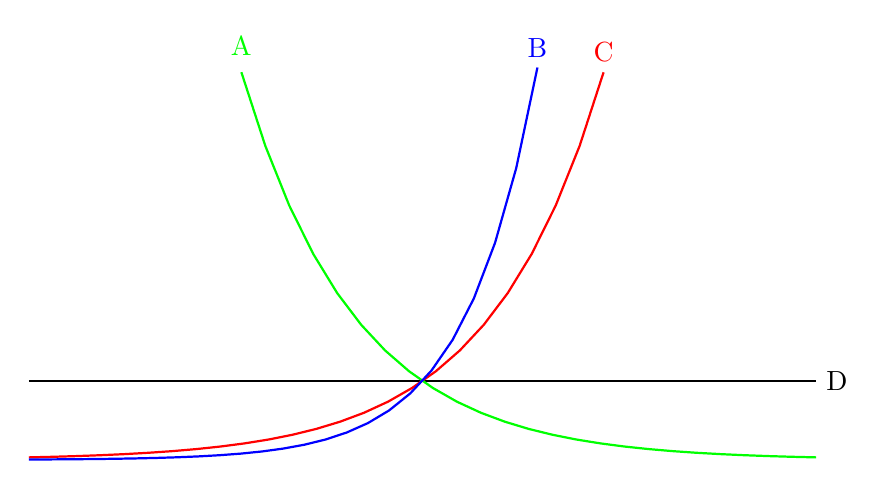
\begin{tikzpicture}
\YEaaxis{5}{5}{1}{5}
\draw[thick] plot[domain=-5:5](\x,1)node[right]{D};%1
\draw[thick, red] plot[domain=-5:2.3](\x,{exp(\x*0.693)})node[above]{C};%2^x
\draw[thick, green] plot[domain=-2.3:5](\x,{1/exp(\x*0.693)});%.5^x
\draw[thick, green] (-2.3,5) node[above]{A};
\draw[thick, blue] plot[domain=-5:1.46](\x,{exp(\x*1.1)})node[above]{B};%3^x
\end{tikzpicture}
\end{center}
\end{Mquestion}
\begin{hint} Two of the functions are the same.
\end{hint}
\begin{answer} A-$(a)$ and $(d)$,\quad B-$(e)$,\quad C-$(c)$,\quad D-$(b)$
\end{answer}
\begin{solution} Since $1^x=1$ for any $x$, we see that $(b)$ is just the constant function $y=1$, so D matches to $(b)$.

Since $2^{-x}=\frac{1}{2^x}=\left(\frac{1}{2}\right)^x$, functions $(a)$ and $(d)$ are the same. This is the only function out of the lot that grows as $x\to-\infty$ and shrinks as $x \to \infty$, so A matches to $(a)$ and $(d)$.

This leaves B and C to match to $(c)$ and $(e)$. Since $3>2$, when $x>0$, $3^x>2^x$. So, $(e)$ matches to the function that grows more quickly to the right of the $x$-axis: B matches to $(e)$, and C matches to $(c)$.
\end{solution}

\begin{Mquestion}
The graph below shows an exponential function $f(x)=a^x$  and its derivative $f'(x)$. Choose all the options that describe the  constant $a$.
\[(a)~a<0\qquad(b)~a>0\qquad\qquad(c)~a<1\qquad(d)~a>1\qquad\qquad(e)~a<e\qquad(f)~a>e\]

\begin{center}
\begin{tikzpicture}
\YEaaxis{5}{5}{1}{5}
\draw[thick, blue] plot[domain=-5:3.97](\x,{exp(\x*0.405)})node[above]{$y=f(x)$};%1.5^x
\draw[thick, red] plot[domain=-5:5](\x,{0.405*exp(\x*0.405)})node[above]{$y=f'(x)$};%1.5^x
\end{tikzpicture}
\end{center}
\end{Mquestion}
\begin{hint}\end{hint}
\begin{answer} $(b),~(d),~(e)$
\end{answer}
\begin{solution}
First, let's consider the behaviour of exponential functions $a^x$ based on whether $a$ is greater or less than 1. As we know,
$\ds\lim_{x\to\infty}a^x=\left\{\begin{array}{ll}
\infty & a>1\\0&a<1
\end{array}\right.$ and $\ds\lim_{x\to-\infty}a^x=\left\{\begin{array}{ll}
0 & a>1\\\infty&a<1
\end{array}\right.$. Our function has $\ds\lim_{x \to \infty} f(x)=\infty$ and
$\ds\lim_{x \to -\infty} f(x)=0$, so we conclude $a>1$: thus $(d)$ and also $(b)$ hold. (We could have also seen that $(b)$ holds because $a^x$ is defined for all real numbers.)

It remains to decide whether $a$ is greater or less than $e$. (If $a$ were equal to $e$, then $f'(x)$ would be the same as $f(x)$.)  We saw in the text that $\diff{}{x}\{a^x\}=C(a)a^x$ for the function $C(a)=\ds\lim_{h \to 0} \dfrac{a^h-1}{h}$. We know that $C(e)=1$. (Actually, we chose $e$ to be the number that has this property.) From our graph, we see that $f'(x)<f(x)$, so $C(a)<1=C(e)$. In other words, $\ds\lim_{h \to 0} \dfrac{a^h-1}{h}<\ds\lim_{h \to 0} \dfrac{e^h-1}{h}$; so, $a<e$. Thus $(e)$ holds.
\end{solution}


\begin{question}
True or false: $\ds\diff{}{x}\{e^x\}=xe^{x-1}$
\end{question}
\begin{hint}
When can you use the power rule?
\end{hint}
\begin{answer}
False
\end{answer}
\begin{solution}
The power rule tells us that $\diff{}{x}\{x^n\}=nx^{n-1}$. In this equation, the variable is the base, and the exponent is a constant. In the function $e^x$, it's reversed: the variable is the exponent, and the base it a constant. So, the power rule does not apply.
\end{solution}



\begin{question}
A population of bacteria is described by $P(t)=100e^{0.2t}$, for $0 \leq t \leq 10$. Over this time period, is the population increasing or decreasing?

\medskip
We will learn more about the uses of exponential functions to describe real-world phenomena in Section~\ref*{sec:ExpGthDecay}.
\end{question}
\begin{hint} What is the shape of the curve $e^{ax}$, when $a$ is a positive constant?
\end{hint}
\begin{answer} increasing
\end{answer}
\begin{solution}
$P(t)$ is an increasing function over its domain, so the population is increasing.

There are a few ways to see that $P(t)$ is increasing.

 What we really care about is whether $e^{0.2t}$ is increasing or decreasing, since an increasing function multiplied by 100 is still an increasing function, and a decreasing function multiplied by 100 is still a decreasing function. Since $f(t)=e^t$ is an increasing function, we can use what we know about graphing functions to see that $f(0.2t)=e^{0.2t}$ is also increasing.
\end{solution}


%%%%%%%%%%%%%%%%%%
\subsection*{\Procedural}
%%%%%%%%%%%%%%%%%%

\begin{question}
Find the derivative of $f(x)=\dfrac{e^{x}}{2x}$
.\end{question}
\begin{hint}
Quotient rule
\end{hint}
\begin{answer}
$\dfrac{(x-1)e^x}{2x^2}$
\end{answer}
\begin{solution}
Using the quotient rule,
\begin{align*}
f'(x)=\frac{2xe^x-2e^x}{4x^2}=\frac{e^x(2x-2)}{4x^2}=\frac{(x-1)e^x}{2x^2}
\end{align*}
\end{solution}

\begin{question}\label{s2.7e2x}
Differentiate $f(x)=e^{2x}$.
\end{question}
\begin{hint}
$e^{2x}=\left(e^x\right)^2$
\end{hint}
\begin{answer}
$2e^{2x}$
\end{answer}
\begin{solution}
\begin{align*}
f'(x)=\diff{}{x}\{e^{2x}\}=\diff{}{x}\{(e^x)^2\}=2\diff{}{x}\{e^x\}e^x=2e^xe^x=2(e^{x})^2=2e^{2x}
\end{align*}
\end{solution}

\begin{question}
Differentiate $f(x)=e^{a+x}$, where $a$ is a constant.
\end{question}
\begin{hint}
$e^{a+x}=e^ae^x$
\end{hint}
\begin{answer}
$e^{a+x}$
\end{answer}
\begin{solution}
\begin{align*}
e^{a+x}&=e^ae^x
\intertext{Since $e^a$ is just a constant,}
\diff{}{x}\{e^{a}e^{x}\}&=e^a\diff{}{x}\{e^x\}=e^ae^x=e^{a+x}
\end{align*}
So, $f'(x)=f(x)=e^{a+x}$.
\end{solution}


\begin{question}
For which values of $x$ is the function $f(x)=xe^x$ increasing?
\end{question}
\begin{hint}
Figure out where the derivative is positive.
\end{hint}
\begin{answer}
$x>-1$
\end{answer}
\begin{solution}
If the derivative is positive, the function is increasing, so let's start by finding the derivative. We use the product rule (although Question~\ref{s2.7expprod} gives a shortcut).
\begin{align*}
f'(x)&=1\cdot e^x+xe^x=(1+x)e^x
\end{align*}
Since $e^x$ is always positive, $f'(x)>0$ when $1+x>0$. So, $f(x)$ is increasing when $x>-1$.
\end{solution}



\begin{Mquestion}
Differentiate $e^{-x}$.
\end{Mquestion}
\begin{hint}
$e^{-x}=\frac{1}{e^x}$
\end{hint}
\begin{answer}
$-e^{-x}$
\end{answer}
\begin{solution}
\begin{align*}e^{-x}&=\frac{1}{e^x}
\intertext{Using the rule for differentiating the reciprocal:}
\diff{}{x}\{e^{-x}\}&=\frac{-e^x}{(e^x)^2}=\frac{-1}{e^x}=-e^{-x}
\end{align*}
\end{solution}

\begin{question}
Differentiate $f(x)=(e^x+1)(e^x-1)$.
\end{question}
\begin{hint}
Product rule will work nicely here. Alternately, review the result of Question~\ref{s2.7e2x}.
\end{hint}
\begin{answer}
$2e^{2x}$
\end{answer}
\begin{solution}
Using the product rule,
\[f'(x)=(e^x)(e^x-1)+(e^x+1)(e^x)=e^x(e^x-1+e^x+1)=2(e^x)^2=2e^{2x}\]

Alternate solution: using Question~\ref{s2.7e2x}:
\[f(x)=e^{2x}-1 \implies f'(x)=2e^{2x}.\]
\end{solution}


\begin{Mquestion}
A particle's position  is given by
\[s(t)=t^2e^t.\]
 When is the particle moving in the negative direction?
\end{Mquestion}
\begin{hint}
To find the sign of a product, compare the signs of each factor. The function $e^t$ is always positive.
\end{hint}
\begin{answer}
When $t$ is in the interval $(-2,0)$.
\end{answer}
\begin{solution}
The question asks when $s'(t)$ is negative. So, we start by differentiating. Using the product rule:
\begin{align*}
s'(t)&=e^t(t^2+2t)\\
&=e^t \cdot t(t+2)
\end{align*}
$e^t$ is always positive, so $s'(t)$ is negative when $t$ and $2+t$ have opposite signs. This occurs when $-2<t<0$.
\end{solution}


%%%%%%%%%%%%%%%%%%
\subsection*{\Application}
%%%%%%%%%%%%%%%%%%

\begin{Mquestion}\label{s2.7expprod}
Let  $g(x)=f(x)e^x$, for a differentiable function $f(x)$. Give a simplified formula for $g'(x)$.


Functions of the form $g(x)$ are relatively common. If you remember this formula, you can save yourself some time when you need to differentiate them. We will explore this more in Question~\ref{s2.14expprod}, Section~\ref*{sec higher diff}.%2.14
\end{Mquestion}
\begin{hint}
After you differentiate, factor out $e^x$.
\end{hint}
\begin{answer}
$g'(x)=[f(x)+f'(x)]e^x$
\end{answer}
\begin{solution}
Using the product rule,
$g'(x)=f'(x)e^x+f(x)e^x=[f(x)+f'(x)]e^x$
\end{solution}


\begin{Mquestion}
Which of the following functions describe a straight line?
\[(a) ~y=e^{3\log x}+1 \qquad (b) ~2y+5=e^{3+\log x} \qquad (c)~y=e^{2x}+4\qquad (d)~y=e^{\log x}3^e+\log 2\]
\end{Mquestion}
\begin{hint}
Simplify
\end{hint}
\begin{answer}
(b) and (d)
\end{answer}
\begin{solution}
We simplify the functions to get a better idea of what's going on.

($a$): $y=e^{3\log x}+1=\left(e^{\log x}\right)^3+1=x^3+1$. This is not a line.
\smallskip

($b$): $2y+5=e^{3+\log x}=e^3e^{\log x}=e^3x$. Since $e^3$ is a constant, $2y+5=e^3x$ is a line.
\smallskip

($c$): There isn't a fancy simplification here--this isn't a line. If that isn't a satisfactory answer, we can check: a line is a function with a constant slope. For our function,
$y'=\diff{}{x}\{e^{2x} +4\}=\diff{}{x}\{e^{2x}\}=\diff{}{x}\left\{(e^x)^2\right\}=2e^xe^x=2e^{2x}$. Since the derivative isn't constant, the function isn't a line.
\smallskip

($d$): $y=e^{\log x}3^e+\log 2=3^e\,x+\log 2$. Since $3^e$ and $\log 2$ are constants, this is a line.
\end{solution}


\begin{question}[2009H]
Find constants $a$, $b$ so that the following function is differentiable:
\[
f(x) =\left\{\begin{array}{ll}
ax^2 + b & x \le 1\\
e^x     &  x > 1\end{array}\right.
\]
\end{question}
\begin{hint}
In order to be differentiable, a function should be continuous. To determine the differentiability of the function at $x=1$, use the definition of the derivative.
\end{hint}
\begin{answer}
$a=b=\dfrac{e}{2}$
\end{answer}
\begin{solution}
When we say a function is differentiable without specifying a range, we mean that it is differentiable over its domain. The function $f(x)$ is differentiable when $x \neq 1$ for any values of $a$ and $b$; it is up to us to figure out which constants make it differentiable when $x=1$.

In order to be differentiable, a function must be continuous. The definition of continuity tells us that, for $f$ to be continuous at $x=1$, we need $\ds\lim_{x \to 1}f(x)=f(1)$. From the definition of $f$, we see $f(1)=a+b=\ds\lim_{x \to 1^-}f(x)$, so we need $\ds\lim_{x\to 1^+}f(x)=a+b$. Since $\ds\lim_{x \to 1^+}f(x)=e^1=e$, we specifically need
\[e=a+b.\]

Now, let's consider differentiability of $f$ at $x=1$. We need the following limit to exist:
\begin{align*}
\lim_{h \to 0} \frac{f(1+h)-f(1)}{h}&
\intertext{In particular, we need the one-sided limits to exist and be equal:}
\textcolor{red}{\lim_{h \to 0^-}\frac{f(1+h)-f(1)}{h}}&=\textcolor{blue}{\lim_{h \to 0^+}\frac{f(1+h)-f(1)}{h}}
\intertext{If $h<0$, then $1+h<1$, so $f(1+h)=a(1+h)^2+b$. If $h>0$, then $1+h>1$, so $f(1+h)=e^{1+h}$. With this in mind, we begin to evaluate the one-sided limits:}
\color{red}\lim_{h \to 0^-}\frac{f(1+h)-f(1)}{h}&\color{red}=
\lim_{h \to 0^-}\frac{[a(1+h)^2+b]-[a+b]}{h}\\
&\color{red}=\lim_{h \to 0^-}\frac{ah^2+2ah}{h}=2a\\
\color{blue}\lim_{h \to 0^+}\frac{f(1+h)-f(1)}{h}&\color{blue}=
\lim_{h \to 0^+}\frac{e^{1+h}-(a+b)}{h}
\intertext{Since we take $a+b$ to be equal to $e$ (to ensure continuity):}
&\color{blue}=
\lim_{h \to 0^+}\frac{e^{1+h}-e^1}{h}\\
&\color{blue}=\left.\diff{}{x}\{e^x\}\right|_{x=1}=e^1=e
\end{align*}

So, we also need
\[\textcolor{red}{2a}=\textcolor{blue}{e}\]

Therefore, the values of $a$ and $b$ that make $f$ differentiable are $a=b=\dfrac{e}{2}$.

%In order for $f$ to be differentiable at $x=1$, it must also
%be continuous at $x=1$. This forces $e^x\big|_{x=1}=\big[ax^2+b\big]_{x=1}$
%or $a+b=e$. In order for $f$ to be differentiable at $x=1$, the right hand
%derivative of $ax^2+b$ at $x=1$, which is $2ax\big|_{x=1}=2a$, must be
%the same as the left hand derivative of $e^x$ at $x=1$, which is
%$e^x\big|_{x=1}=e$. So we need
%$$
%a+b=e,\ 2a=e\implies a=b=\frac{e}{2}
%$$
\end{solution}
